\begin{tikzpicture}[node distance=6ex and 4ex, every node/.style={font=\small}]
% BEGIN ROW 1
\umlclassvarwidth[]{eme}{[]}{\itshape EModelElement}{%
}{13ex}
\umlclassvarwidth[]{ene}{[base right=of eme]}{\itshape ENamedElement}{%
name:String
}{15ex}
\umlsuperclassof{eme.east}{
--
}{ene.west |- eme.east}
\umlclassvarwidth[]{ete}{[base right=of ene]}{\itshape ETypedElement}{%
lowerBound:int\newline
upperBound:int\newline
ordered:bool
}{16ex}
\umlsuperclassof{ene.east}{
--
}{ete.west |- ene.east}
% BEGIN ROW 2
\umlclassvarwidth[,yshift=2ex]{ecf}{[below=of ene]}{\itshape EClassifier}{%
}{15ex}
\umlassociationfromto{
(ete.south)
|-
node[pos=1,above right] {eType}
node[pos=1,below right=0.5ex and 0ex] {0..1}
($(ecf.east)+(0,-2ex)$)
}
\umlsuperclassof{ene.south}{
--
}{ecf.north}
\umlclassvarwidth[]{eel}{[base left=of ecf]}{EEnumLiteral}{%
}{13ex}
\umlsubclassof{eel.north}{
-- ++ (0ex,2ex)
-|
}{ene.south}
% BEGIN ROW 3
\umlclassvarwidth[]{ee}{[below=of eel]}{EEnum}{%
}{13ex}
\umlcomposition{%
(ee.north)
-- 
node[pos=1,below left] {eLiterals}
node[pos=1,below right] {0..*}
(eel)
}
\umlclassvarwidth[]{edt}{[base right=of ee]}{EDataType}{%
}{15ex}
\umlsuperclassof{edt.west}{
--
}{ee.east}
\umlsuperclassof{ecf.south}{
--
}{edt.north}
\umlclassvarwidth[]{ec}{[base right=of edt]}{EClass}{%
abstract:bool
}{16ex}
\umlsubclassof{$(ec.north)+(-8ex,0)$}{
-- ++(0,2ex)
-|
}{ecf.south}
\umlsuperclassof{edt.east}{
--
}{ec.west |- edt.east}
\umlassociationfromto{
($(ec.north)+(-6ex,0)$)
-- ++(0,3ex)
-- ++(6ex,0)
-- ++(0,-3ex)
node[pos=1,above right=-0.2ex and 0.5ex] {eSuperTypes}
node[pos=1,above left=-.1ex and 0.5ex] {0..*}
}
% BEGIN ROW 4
\umlclassvarwidth[]{esf}{[below=of ec, yshift=-3ex]}{\itshape EStructuralFeature}{%
abstract:bool
}{16ex}
\umlcomposition{%
($(ec.south)+(6ex,0)$)
-- 
node[pos=1,above left] {eStructuralFeatures}
node[pos=1,above right] {0..*}
++(0,-9ex)
}
\umlsuperclassof{ete.east}{
-- ++(3.5ex,0)
|-
}{esf.east}
\umlclassvarwidth[]{er}{[base left=of esf]}{EReference}{%
containment:bool
}{15ex}
\umlassociationfromto{
(er.north)
-- ++(0,4.5ex)
-|
($(ec.south)+(-8.5ex,0)$)
node[pos=.85,below left] {/eReferenceType}
node[pos=.85,below right] {1}
}
\umlsuperclassof{esf.south}{
-- ++(0,-3ex)
-|
}{er.south}
\umlclassvarwidth[]{ea}{[base left=of er]}{EAttribute}{%
id:bool
}{13ex}
\umlassociationfromto{
(ea.north)
-- ++(0,6ex)
-|
($(edt.south)+(-6ex,0)$)
node[pos=.95,below left] {/eAttributeType}
node[pos=.95,below right] {1}
}
\umlsuperclassof{esf.south}{
-- ++(0,-3ex)
-|
}{ea.south}
\end{tikzpicture}